% METODOLOGIA------------------------------------------------------------------
\chapter{PROCEDIMENTOS METODOLÓGICOS}
\label{chap:metodologia}

Este capítulo tem como finalidade descrever a metodologia e os procedimentos adotados na confecção deste projeto, bem como também realizar uma consolidação de todos os métodos aqui utilizados e apresentar o funcionamento do sistema como um todo.  A figura abaixo mostra um diagrama contendo os diferentes módulos que compõem o projeto:

\begin{figure}[H]
    \centering
    \caption{Diagrama geral da planta de controle}
    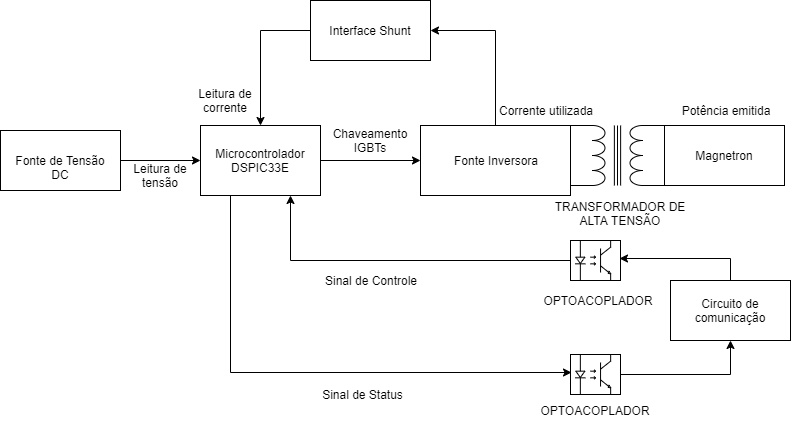
\includegraphics[width=1\textwidth]{./dados/figuras/overall_diagram}
    \fonte{Autoria Própria}
    \label{fig:figura-overall_diagram}
\end{figure}


Assim, cada módulo será detalhado nas seções que seguem à este capítulo. Para tal, os procedimentos metodológicos foram divididos da seguinte forma: Fonte inversora (Seção 3.1), Fonte de alimentação (Seção 3.2),  Realimentação de corrente (Seção 3.3), DSPIC33  (Seção 3.4), Circuito de comunicação (Seção 3.5), Montagem dos circuitos (Seção 3.6), Planta (seção 3.7).

\section{FONTE INVERSORA}
\label{sec:fonteInversora}

Para realizar a alimentação do magnetron, foi utilizada uma fonte inversora, a qual consiste em um inversor ressonante classe E. Segundo \citeonline{Hidenori1991}, uma fonte inversora tem as seguintes vantagens em relação à uma fonte ferrorressonante tradicional:
\begin{itemize}
    \item Potência de saída controlável;
    \item Maior eficiência energética;
    \item Circuito menor e mais leve;
    \item Pode operar em maior frequência.
\end{itemize} 

\begin{figure}[!htb]
    \centering
    \caption{Fonte inversora para alimentação do magnetron}
    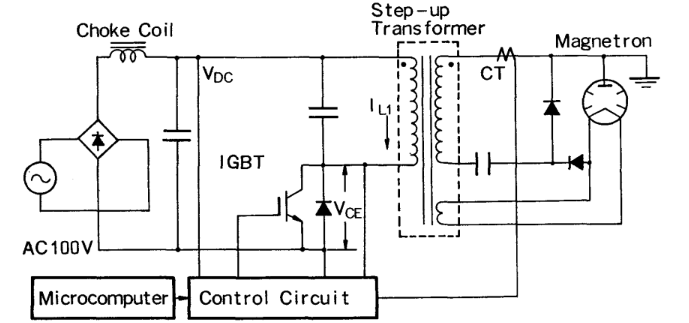
\includegraphics[width=0.9\textwidth]{./dados/figuras/font_inverter}
    \fonte{\citeonline{Hidenori1991}}
    \label{fig:figura-inverter}
\end{figure}

\subsection{Simulações}
\label{sec:simulations}

Para verificar se a fonte inversora é viável para o projeto, foram feitas simulações do circuito no software \textit{PSIM}. Na alimentação o magnetron, são necessários cerca de 4 kV. Assim, primeiramente foi desenvolvido um circuito para simular a alimentação de uma carga de cerca de 100 M$\Omega$, com uma tensão de entrada de 127 V. A figura a seguir mostra o circuito desenvolvido:

\begin{figure}[!htb]
    \centering
    \caption{Circuito da fonte inversora simulada}
    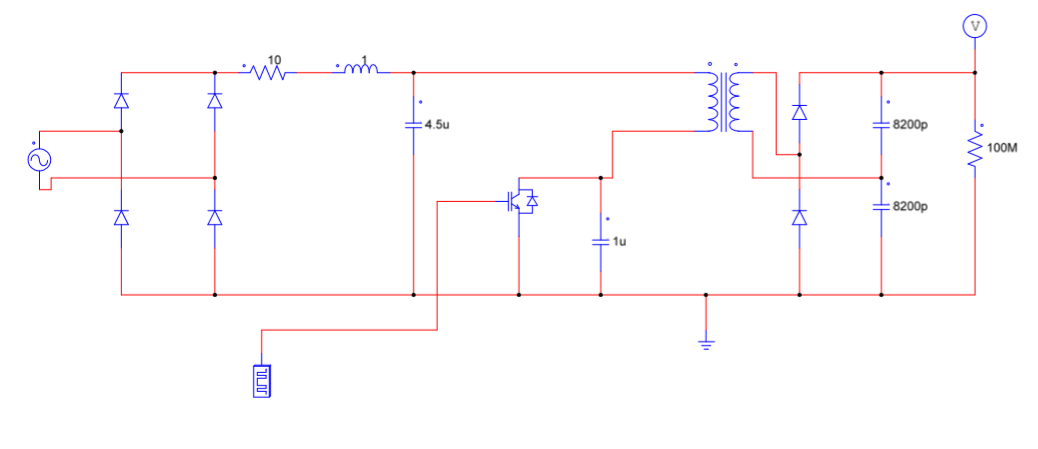
\includegraphics[width=0.9\textwidth]{./dados/figuras/psim1}
    \fonte{Autoria própria (2019)}
    \label{fig:circ_sim_1}
\end{figure}

Para averiguar se uma fonte inversora consegue alimentar uma carga de alta potência à uma tensão de alguns kV, o inversor foi chaveado em um ciclo de trabalho de 50\%. A figura abaixo mostra a forma de onda da tensão na carga resistiva:

\begin{figure}[!htb]
    \centering
    \caption{Forma da onda simulada da tensão na carga}
    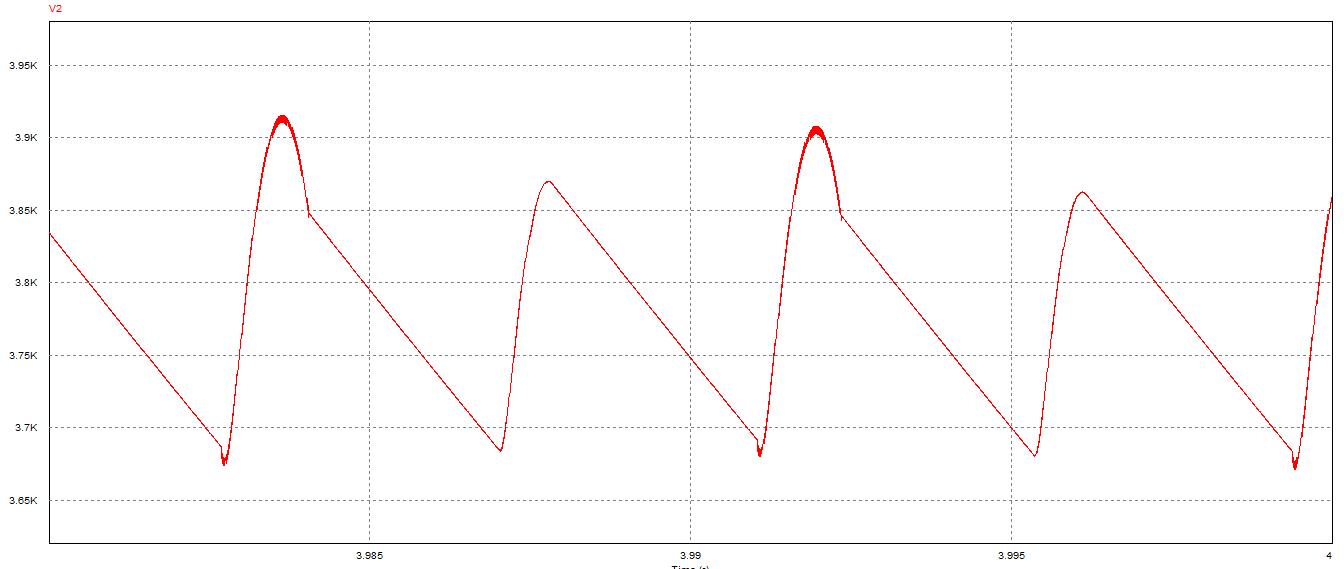
\includegraphics[width=0.9\textwidth]{./dados/figuras/psim2}
    \fonte{Autoria própria (2019)}
    \label{fig:figura-graf_sim_1}
\end{figure}

Na figura \ref{fig:figura-graf_sim_1}, pode-se ver que o pico de tensão da carga chega à quase 4 kV, o que já é suficiente para o objetivo em questão. Logo, conclui-se que a fonte inversora é viável para a alimentação do circuito de um magnetron.

\subsection{Projeto}

O projeto da fonte inversora se baseou em boa parte no conceito desenvolvido por \citeonline{Hidenori1991}. Assim como no circuito implementado pelos engenheiros japoneses, a equipe baseou o projeto da fonte em um inversor classe E e o chaveamento do circuito é feito por um microcontrolador. Devido à operação em alta frequência do sistema, o CI IR1153S foi usado para aplicar uma correção do fator de potência, diminuindo significativamente a taxa de distorção harmônica (TDH). Para uma maior eficiência, foram utilizados IGBTs em paralelo para aumentar a potência dos sistemas e reduzir as perdas no circuito. Um transformador de três enrolamentos de alta potência, em conjunto com um circuito dobrador, alimenta as entradas do magnetron. O polo positivo de um dos enrolamentos do secundário do transformador é ligado ao terra e o polo negativo é ligado ao ânodo do magnetron. No primeiro enrolamento, o pólo negativo está em curto-circuito com o lado positivo do segundo enrolamento e o pólo positivo está ligado ao cátodo do magnetron. Com esta montagem, a tensão de entrada do magnetron é cerca de 4kV. A tensão de entrada do circuito é a tensão da rede retificada por uma ponte de diodos. O esquemático do circuito foi desenvolvido no software \textit{Altium Desginer}. A figura \ref{fig:proj-font-inv} mostra o circuito projetado:

\begin{figure}[!htb]
    \centering
    \caption{Circuito projetado}
    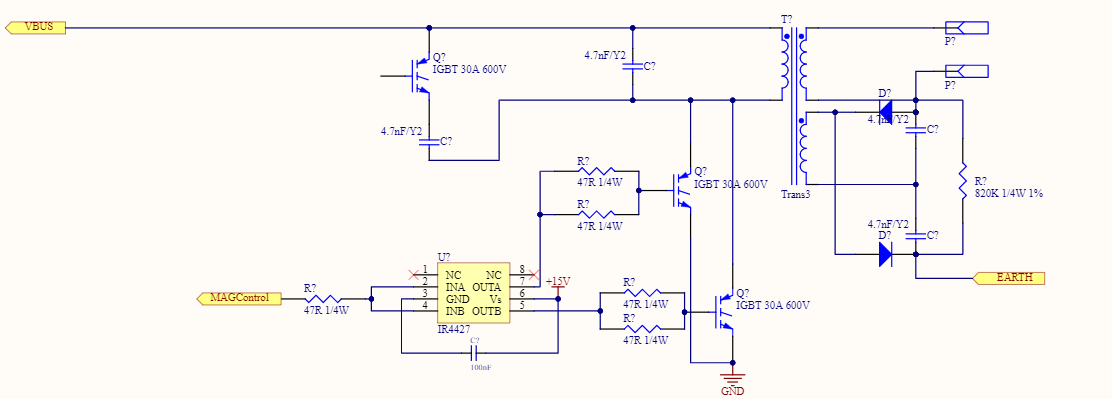
\includegraphics[width=1.1\textwidth]{./dados/figuras/proj-font-inv}
    \fonte{Autoria própria (2019)}
    \label{fig:proj-font-inv}
\end{figure}

\subsection{Descrição de funcionamento}
O circuito é projetado para permitir o controle da potência de saída do magnetron, cujos terminais são conectados aos conectores P3 e P4, os quais estão ligados na saída do secundário do transformador. Os diodos D8 e D9, juntamente com os capacitores C22 e C24 formam um circuito dobrador,  permitindo que o pico da tensão de saída chegue em aproximadamente 4 kV. O controle de potência é feito pelo chaveamento conjunto dos IGBTs Q4 e Q5, os quais controlam a passagem de corrente pelo \texit{shunt}. O chaveamento destes dispositivos é feito por um microcontrolador, que controla o chaveamento de acordo com o valor de corrente lido nos terminais do resistor \textit{shunt}. Quanto maior a corrente neste resistor, maior a potência de entrada do magnetron. O IGBT Q3, juntamente com os diodos D10, D11, D12 e a rede de resistores consistem em um circuito que exerce o mesmo papel de um diodo roda-livre. Este circuito bloqueia os picos de tensão induzida gerada pelo transformador quando os IGBTs Q4 e Q5 são despolarizados.
Diferentemente do projeto do circuito  da figura \ref{fig:figura-inverter}, o circuito desenvolvido não utiliza um CI para realizar as ações determinadas pelo microcontrolador. No trabalho desenvolvido pela equipe, a realimentação é feita pelo resistor \textit{shunt} ligado ao neutro, em vez do transformador de corrente. Assim, a leitura do valor da corrente pode ser feita por um simples condicionamento do sinal, utilizando uma interface que utiliza resistores, capacitores e um amplificador operacional integrado ao microcontrolador. O CI U7, além de diminuir a TDH, também faz o isolamento do sinal que vem do microcontrolador do resto do circuito. Portanto, optou-se por não utilizar um circuito de controle especializado.



\section{\texit{FONTE DE ALIMENTAÇÃO}}
\label{sec:font}

 Para alimentar os diferentes componentes do sistema, utilizou-se um projeto de fonte de alimentação isolada, com potência de 10W. A fonte utilizada possui saídas de 3,3V e 15V, utilizando reguladores chaveados para manter o sinal de tensão o mais constante possível. A equipe fez uma modificação no circuito para energizar o inversor que faz o controle de potência do magnetron com a tensão após a ponte de diodos. Outra mudança feita foi o posicionamento de um resistor \textit{shunt}, ligado ao neutro do circuito. Este componente atua como um sensor de corrente que é usado na função de transferência da realimentação da planta. A alimentação do inversor é feita com o sinal de tensão da saída do indutor ligado ao retificador de onda completa. Também foi adicionada uma série de resistores que são utilizados em um divisor de tensão que é ligado a um conversor AD do microcontrolador. A tensão medida no resistor R20 é utilizada no cálculo da potência utilizada pelo circuito. Na fonte, foram utilizados quatros CIs especializados. O CI TNY274PN é um regulador chaveado e isolado, que permite abaixar para o valor desejado de 15 V uma ampla faixa tensão de entrada DC. Este dispositivo é um dos mais flexíveis do mercado, permitindo o uso de uma maior potência na tensão de entrada, reduzindo os custos com o transformador da fonte. Para chegar à tensão de 3,3 V, foi utilizado o CI L78L33AC, que é um regulador de tensão fixa. Este CI emprega um limitador de corrente que inibe qualquer sobrecarga que a fonte venha a apresentar na saída. Para fazer o acoplamento do regulador chaveado, foi utilizado o optoacoplador PC817. Este modelo é um dos mais comuns para aplicações que precisam isolar dois circuitos com diferentes potências e impedâncias. Para proteger o circuito, foi usado o CI TL431, que exerce a mesma função de um diodo zener, protegendo o circuito em uma eventual sobrecarga. A figura abaixo mostra o esquemático da fonte de alimentação utilizada:

\begin{figure}[H]
   \centering
   \caption{Fonte de alimentação do sistema}
    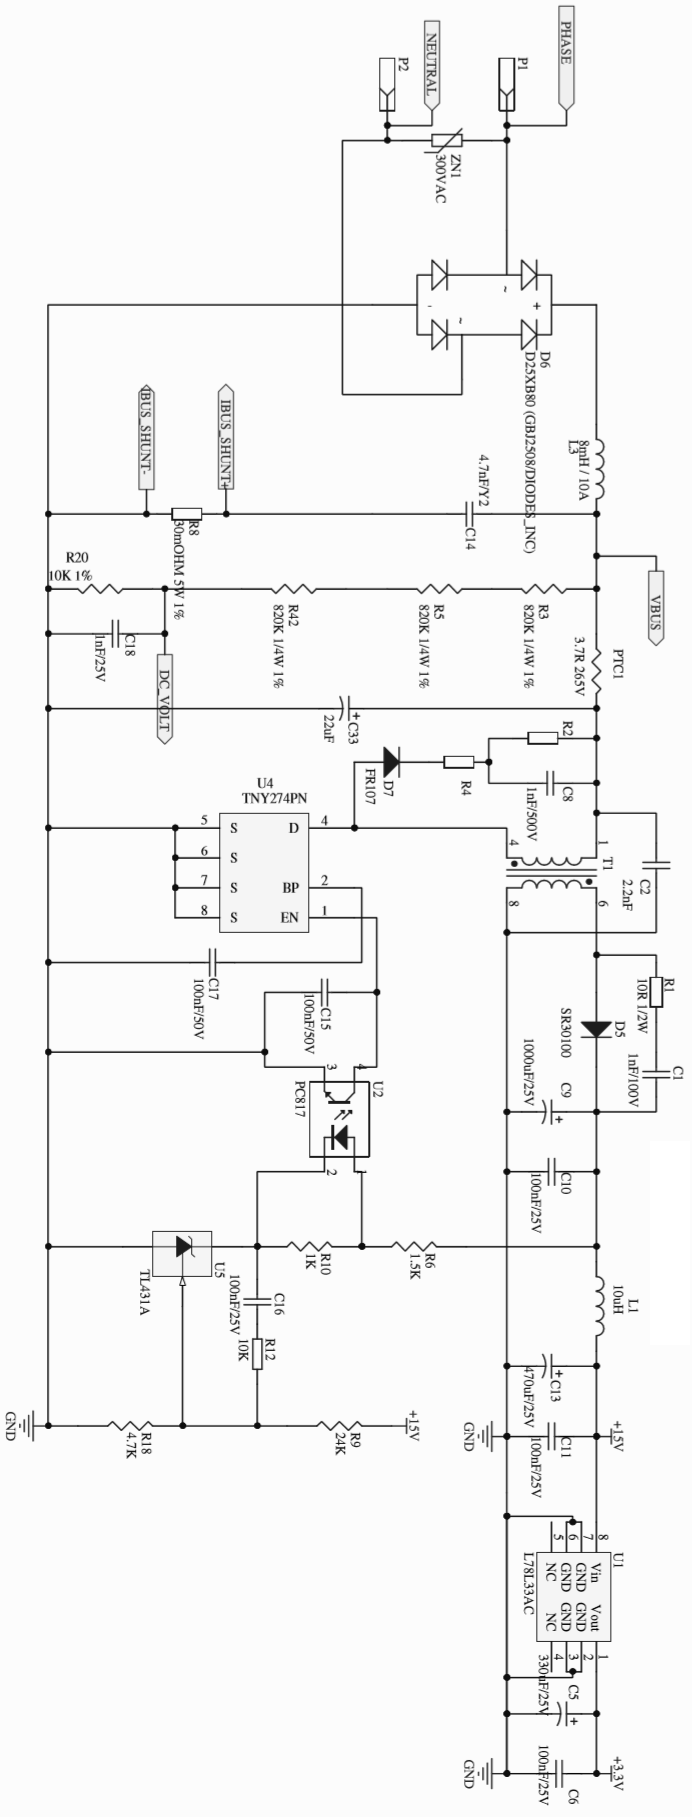
\includegraphics[width=0.55\textwidth]{./dados/figuras/proj-font-alim}
    \fonte{Autoria própria (2019)}
    \label{fig:proj-font-alim}
\end{figure}

\pagebreak


\section{\texit{REALIMENTAÇÃO DE CORRENTE}}
\label{sec:shunt}
No trabalho apresentado por \citeonline{Hidenori1991}, a planta de controle de potência do magnetron utiliza uma realimentação de corrente, através de um transformador de corrente na saída do secundário do transformador de alta tensão. No entanto, esta abordagem causa distorção no circuito. Como a corrente que circula no sistema está diretamente relacionada à potência fornecida pelo magnetron, a realimentação de corrente foi escolhida como solução, porém a equipe decidiu utilizar uma técnica que utiliza um resistor \textit{shunt}.

 Para possibilitar esta realimentação, foi desenvolvida uma interface analógica que é ligada diretamente ao ADC do microcontrolador. A interface consiste em um circuito que, em conjunto com um amplificador operacional integrado ao microcontrolador, irá condicionar o sinal da tensão aplicada em um resistor \textit{shunt} de 30 m$\Omega$ para os pinos de \textit{input} do microcontrolador. A figura abaixo mostra a interface projetada:

\begin{figure}[!htb]
    \centering
    \caption{Condicionador de sinal de realimentação}
    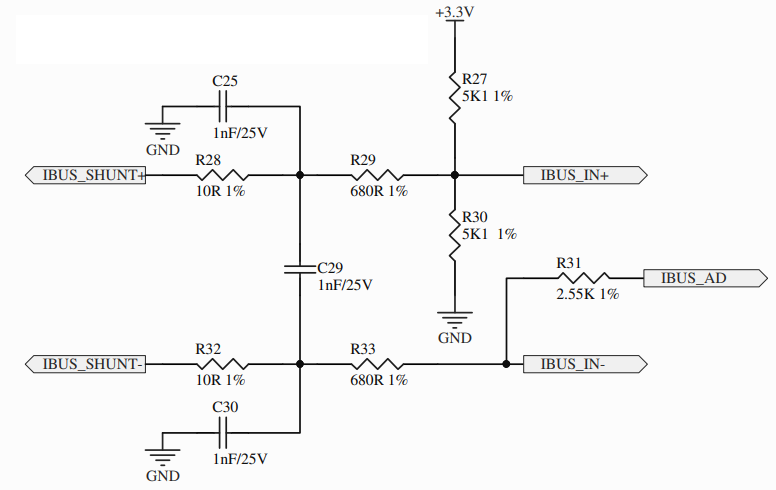
\includegraphics[width=0.9\textwidth]{./dados/figuras/proj-shunt}
    \fonte{Autoria própria (2019)}
    \label{fig:proj-shunt}
\end{figure}


\section{DSPIC33}
\label{sec:dsPIC}

O DSPIC33 é um microcontrolador da família PIC, desenvolvido pela Microchip Technology Inc., que possui funcionalidade de processador digital de sinais (DSP). Este componente foi escolhido para fazer o controle do chaveamento da fonte inversora pois consegue operar em uma ampla faixa de temperatura e possui diversas funcionalidades interessantes para o controle de sinais analógicos de alta frequência. Algumas das funcionalidades, cruciais para o projeto, incluem:

\begin{itemize}
    \item Módulo ADC configurável de 10 bits e amostragem de 1.1 Msps ou 12 bits e amostragem de 500 ksps;
    \item Três amplificadores operacionais integrados ao ADC da plataforma;
    \item Interrupções de \textit{Input Capture} em todos os pinos de I/O;
    \item \textit{Timers} e contadores de 32 bits;
    \item Funções de PWM de alta velocidade.
\end{itemize} 

A CPU da plataforma possui arquitetura Harvard, típica da família de processadores PIC, possuindo uma palavra de instrução de 24 bits e 12 MB de endereços de memória de programa. O microprocessador possui um extenso suporte ao processamento digital de sinais, tendo acumuladores e ULA de 40 bits, dois multiplicadores de alta velocidade 17 por 17 bits e um \textit{barrell shifter} de 40 bits que consegue alternar 16 bits em único ciclo de \textit{clock}. A arquitetura do processador fornece uma compilação eficiente de código, suportando a linguagem C e \textit{Assembly}.

No circuito, o microcontrolador recebe o sinal digital de corrente  condicionado da saída do amplificador operacional integrado, que por sua vez tem as entradas ligadas à interface do \textit{shunt}. O dispositivo também faz uma conversão analógica digital do sinal de tensão de um resistor do divisor de tensão de entrada. Os sinais digitais são convertidos em valores analógicos equivalentes e utilizados para calcular a potência utilizada e a corrente total utilizada pelo circuito. De acordo com os valores medidos, o microcontrolador faz o chaveamento dos IGBTs.

\begin{figure}[H]
    \centering
    \caption{Esquemático do microcontrolador no circuito}
    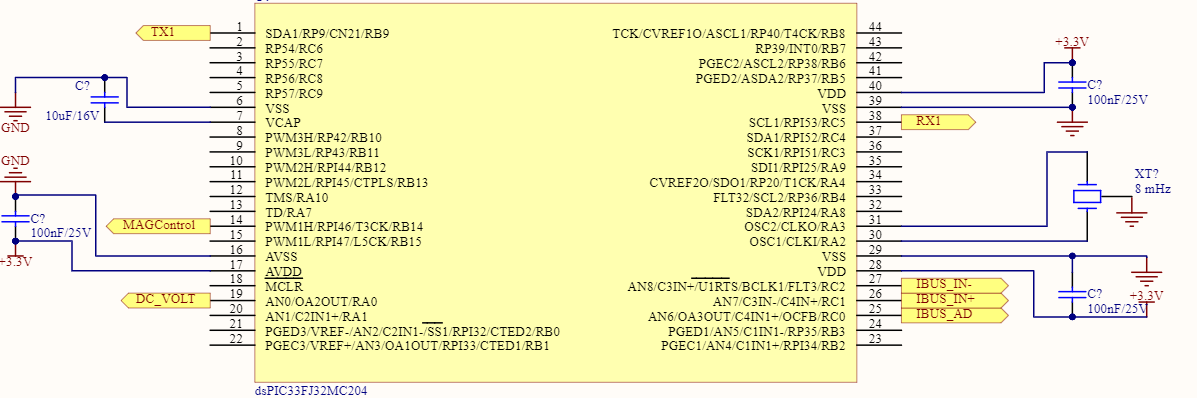
\includegraphics[width=0.9\textwidth]{./dados/figuras/proj-uc}
    \fonte{Autoria própria (2019)}
    \label{fig:figura-dspic}
\end{figure}


\section{CIRCUITO DE COMUNICAÇÃO}
\label{sec:commCircuit}
O circuito de comunicação é responsável por receber sinais de status e enviar sinais de controle para o microcontrolador. Estes sinais de controle podem ser gerados a partir de uma ação do usuário em uma interface externa ou podem ser uma decisão do próprio algoritmo do processador. Para permitir a comunicação do microcontrolador com componentes de alta potência, desenvolveu-se um circuito de comunicação que faz a transmissão e recepção de dados. A interface envia dados para o microcontrolador, contendo sinais de controle, os quais determinam o percentual de potência máxima solicitada, enquanto o microcontrolador envia os sinais de status que sinalizam o estado da realimentação. Este circuito utiliza optoacopladores para fazer a transmissão e recepção dos dados e apresenta uma saída de três conectores que são conectadas à saídas digitais. O  optoacoplador utilizado foi o modelo K10101A, da marca Cosmo Electronics. Este circuito integrado possui frequência de operação de até 80 kHz, que é mais que suficiente para o projeto, dado que os sinais de controle não necessitam de uma alta taxa de transmissão. O esquemático abaixo mostra o circuito de comunicação:

\begin{figure}[H]
    \centering
    \caption{Esquemático do circuito de comunicação}
    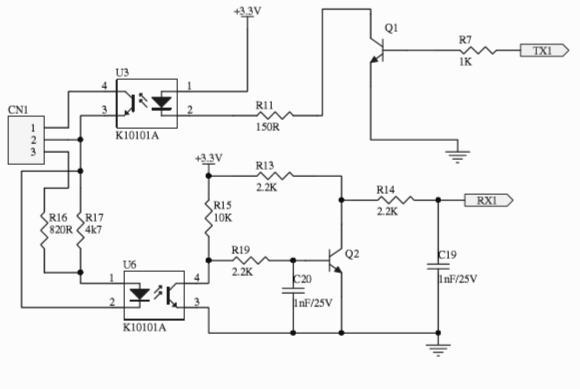
\includegraphics[width=0.9\textwidth]{./dados/figuras/proj-comm}
    \fonte{Autoria própria (2019)}
    \label{fig:figura-comm}
\end{figure}



\section{MONTAGEM DOS CIRCUITOS}
\label{sec:montagem}
Após desenvolver todos os circuitos que compõe a planta que controla a potência de saída do magnetron, a integração dos diferentes componentes foi feita. Para economizar espaço e deixar a montagem mais robusta, foi desenvolvido um esquemático de PCB que contém todas as partes desenvolvidas, usando tanto componentes comerciais comuns quanto componentes SMD. O projeto da placa levou em consideração as altas frequências que são usadas no sistema e o objetivo de o reduzir peso e espaço adicionais presentes em um circuito de forno microondas comum. A figura abaixo mostra o esquemático da PCB desenvolvida no \textit{Altium Designer}.

\begin{figure}[H]
    \centering
    \caption{Esquemático da PCB desenvolvida}
    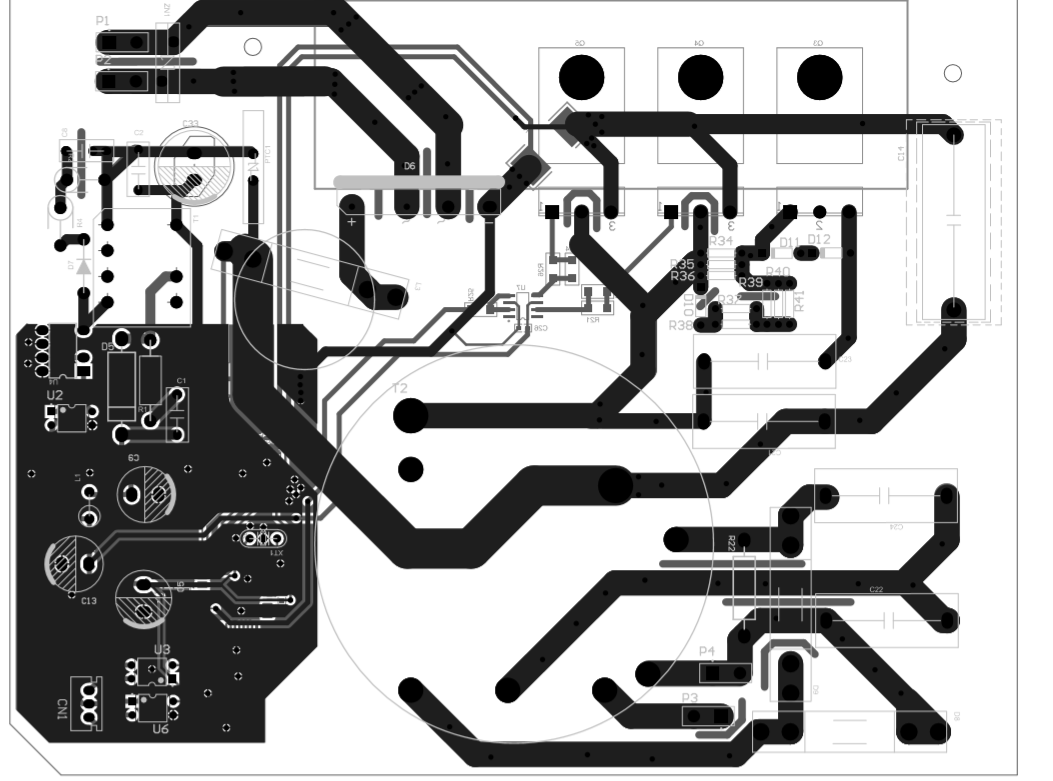
\includegraphics[width=0.9\textwidth]{./dados/figuras/proj-pcb}
    \fonte{Autoria própria (2019)}
    \label{fig:figura-montagem}
\end{figure}

\subsection{Fonte de Tensão}
Para montar a fonte de tensão, foram consideradas as condições de operação do sistema e os objetivos deste trabalho. A placa deve ser compacta, reduzindo o espaço que seria ocupado pelo circuito tradicional, que utiliza um transformador ferrorressonante. A fonte de tensão foi montada utilizando componentes disponíveis no comércio, incluindo componentes SMD. Em vez de utilizar quatro diodos para fazer a ponte retificadora, utilizou-se um CI de 4 pinos que faz a mesma função, utilizando bem menos espaço, sendo acoplável ao dissipador.  A fonte possui duas saídas isoladas de tensão contínua, de 3,3 V e 15 V, para permitir a devida alimentação dos diferentes componentes do sistema. O dissipador precisa de tamanho suficiente para dissipar o calor gerado pela retificação da tensão da rede e o chaveamento dos três IGBTs da fonte inversora. Segue a imagem dos componentes da placa montada:

\begin{figure}[H]
    \centering
    \caption{Placa montada}
    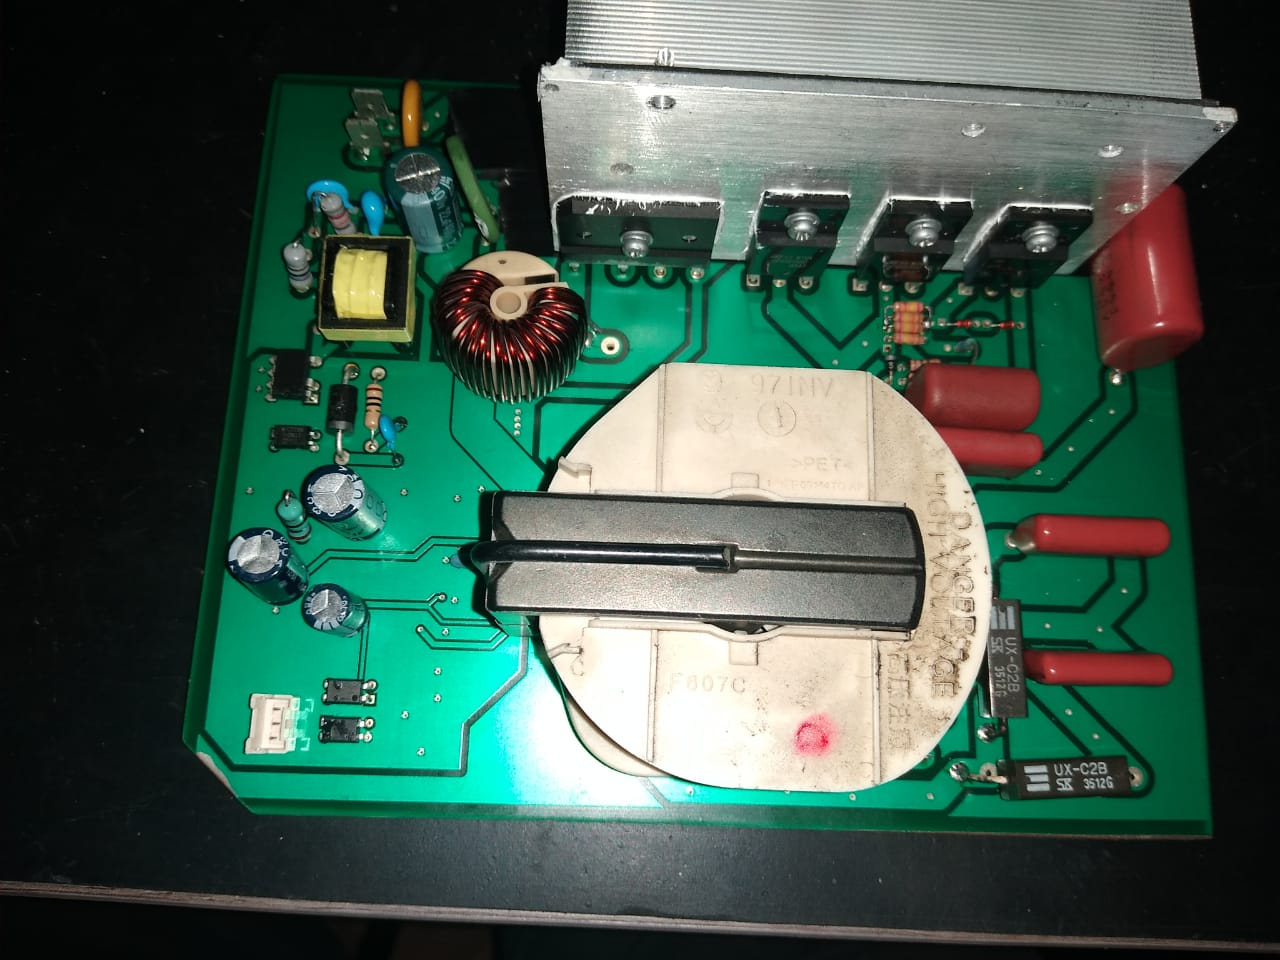
\includegraphics[width=0.9\textwidth]{./dados/figuras/placa_hv}
    \fonte{Autoria própria (2019)}
    \label{fig:figura-montagem-font}
\end{figure}

Em destaque na imagem, vê-se o dissipador, com a ponte de diodos parafusada mais à esquerda.  Logo a frente do retificador onda completa, pode-se ver o indutor de estrangulamento, o qual bloqueia altas frequências indesejadas. À esquerda do indutor, vê-se o transformador que diminui a tensão de para o nível adequado às saídas utilizadas.  Para os resistores e capacitores, foram utilizados componentes comuns, com tensão e potência de operações que variam de acordo com a necessidade. O tipo do capacitor também varia, utilizando-se os tipos de poliester, eletrolítico e tântalo.

\subsection{Circuito de Comunicação}
O circuito de comunicação foi montado com capacitores eletrolíticos e resistores comerciais. Os transistores e opto-acopladores utilizados são de modelos de comum utilização em aplicações de baixa potência. A figura \ref{fig:figura-montagem-comm} destaca onde os componentes desse circuitos foram montados na placa:

\begin{figure}[H]
    \centering
    \caption{Placa montada destacando circuito de comunicação}
    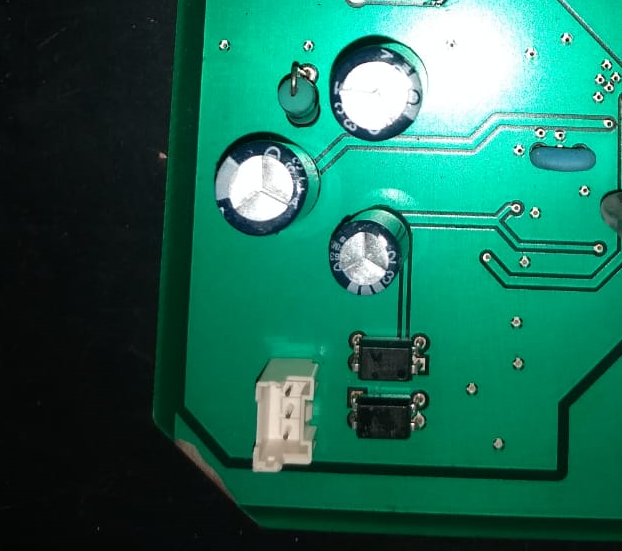
\includegraphics[width=0.9\textwidth]{./dados/figuras/placa_comm.png}
    \fonte{Autoria própria (2019)}
    \label{fig:figura-montagem-comm}
\end{figure}

Na parte de baixo do circuito, pode-se enxergar os dois opto acopladores do circuito e, ao lado deles, vê-se os conectores do sinal de controle. Os resistores do circuito são do tipo SMD, e estão na parte de baixo da placa.

\subsection{Shunt e Microcontrolador}
Para montar a interface que condiciona o sinal dos terminais do shunt à entrada do ADC, foram utilizados componentes comuns. Devido a um erro da equipe na hora de soldar os componentes e o microcontrolador, os pontos originais de solda do circuito foram perdidos. Para não ter que refazer a placa, os componentes foram soldados diretamente uns aos outros com jumpers. Para fixar os objetos, utilizou-se cola quente. O \textit{package} microcontrolador é do tipo PLCC. Segue a foto da montagem do circuito:

\begin{figure}[H]
    \centering
    \caption{Montagem da interface \texit{shunt} e do microcontrolador}
    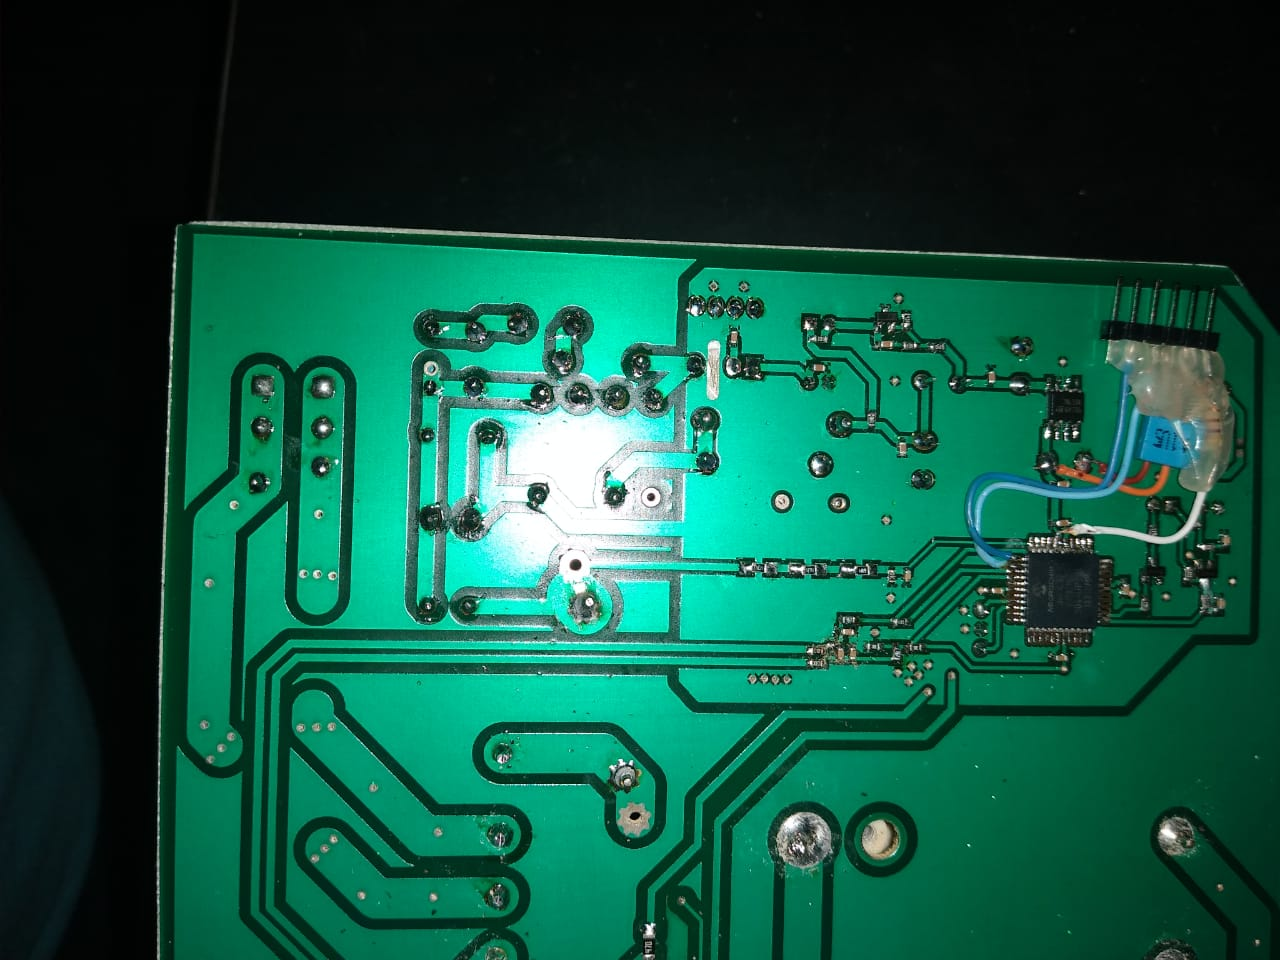
\includegraphics[width=0.9\textwidth]{./dados/figuras/placa_shunt}
    \fonte{Autoria própria (2019)}
    \label{fig:figura-montagem-shunt-uc}
\end{figure}

\subsection{Fonte Inversora}
Na fonte inversora, foram utilizados capacitores de poliéster de alta tensão, resistores comuns e IGBTs 30A, 600V do modelo 1MBH50D, da marca Fuji. O transformador é um modelo de três enrolamentos, com um enrolamento no lado primário e dois enrolamentos no lado secundário. O enrolamento do lado primário é constituído com 19 voltas de um fio de cobre flexível com espessura de 3mm. Um dos enrolamentos do lado secundário é constituído por 270 voltas. Este lado é o lado que é ligado ao circuito dobrador. Já o outro enrolamento, possui apenas uma volta, cuja função é polarizar o magnetron.

\begin{figure}[H]
    \centering
    \caption{Montagem da fonte inversora}
    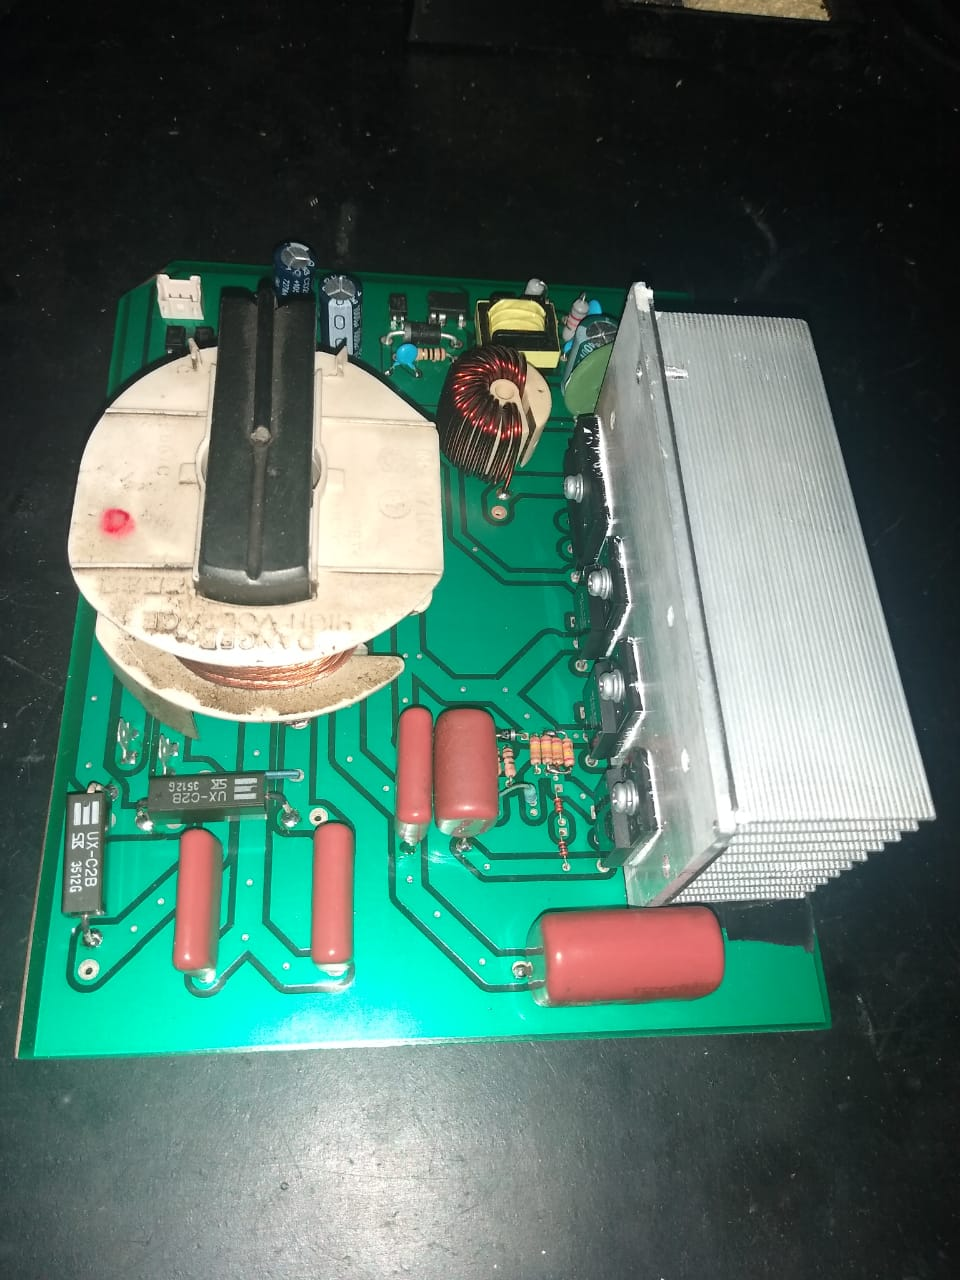
\includegraphics[width=0.9\textwidth]{./dados/figuras/montagem-inverter}
    \fonte{Autoria própria (2019)}
    \label{fig:figura-montagem-inverter}
\end{figure}

Na figura \ref{fig:figura-montagem-inverter} destaca-se o transformador de alta tensão à esquerda. Logo abaixo dele, pode-se ver o circuito dobrador, com os capacitores C22 e C24, da figura \ref{fig:proj-font-inv}, e os diodos de alta potência. O diodo utilizado foi o modelo UX-C2B. Este modelo é adequado para este tipo de aplicação pois suporta tensões de até 8,5 kV e possui uma baixa taxa de polarização direta. Os dois conectores logo abaixo do transformador, do lado esquerdo são conectados aos terminais do magnetron. À direita do dobrador, vê-se o circuito roda livre, ao lado esquerdo dos dois IGBTs que fazem o chaveamento do circuito. Para o circuito roda-livre, foi utilizado o mesmo modelo de IGBT que é utilizado no controle de potência, uma rede resistiva de resistores comerciais comuns, com três diodos também comuns. Devido ao uso de um chassi metálico no forno microondas, o lado positivo do enrolamento de 270 fios do secundário é ligado ao terra. 

\subsection{Magnetron}
O magnetron utilizado no projeto é um magnetron comum, disponível em microondas domésticos. O dispositivo foi fabricado pela empresa Panasonic, e foi retirado de um modelo de microondas da mesma marca. Segue a foto do magnetron utilizado:

\begin{figure}[H]
    \centering
    \caption{Magnetron utilizado}
    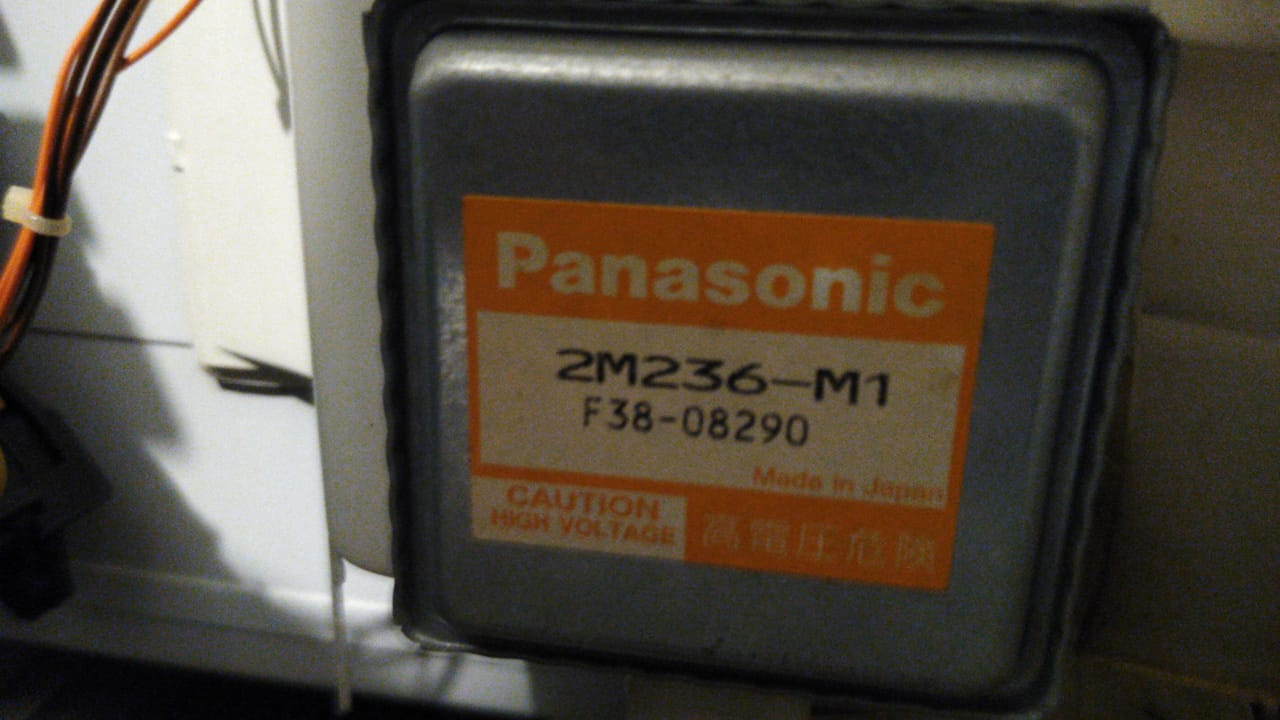
\includegraphics[width=0.9\textwidth]{./dados/figuras/magnetron-usado}
    \fonte{Autoria própria (2019)}
    \label{fig:figura-magnetron-usado}
\end{figure}

\subsection{Montagem completa}
A montagem completa utilizou um forno microondas da marca Panasonic do ano 1995. A fonte ferrorressonante de alimentação do magnetron foi retirada, e trocada pela placa montada desenvolvida pela equipe. O magnetron do forno utilizado foi preservado. A imagem abaixo mostra a montagem completa:
\begin{figure}[H]
    \centering
    \caption{Montagem completa}
    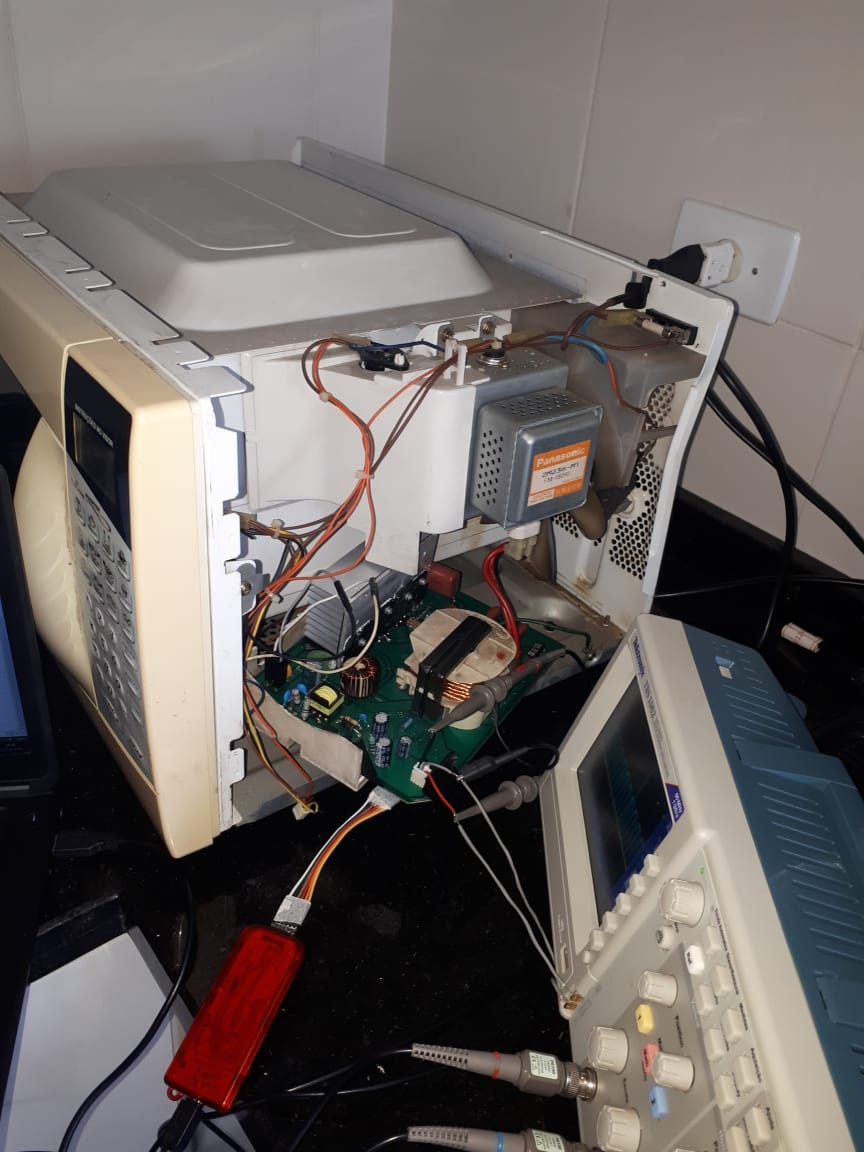
\includegraphics[width=0.9\textwidth]{./dados/figuras/montagem-full}
    \fonte{Autoria própria (2019)}
    \label{fig:figura-montagem-shunt-uc}
\end{figure}

\section{PLANTA}
\label{sec:plant}
Para fazer o controle de potência de saída do magnetron, foi projetada uma planta que possibilita o ajuste da potência ao \textit{set point} requerido. Para tal, foram desenvolvidos circuitos e algoritmos para microcontrolador de modo que o controle fosse realizado através do chaveamento dos IGBTs, utilizando realimentação de corrente pelo resistor \textit{shunt}. A estratégia de controle adotada foi o uso de um controlador proporcional integral (PI). Para controlar a potência de saída, o microcontrolador chaveia dois IGBTs, variando dois parâmetros: ciclo de trabalho e frequência do pulso. Para a leitura do valor do \textit{shunt}, foi utilizado um conversor AD e um amplificador operacional, ambos integrados ao microcontrolador. Para medir a tensão do barramento de tensão da rede retificada (Vbus), também foi utilizado um conversor AD integrado ao microcontrolador. Esta tensão é usada tanto no cálculo realizado para o controle potência de saída quanto para medir a potência utilizada pelo circuito.

\subsection{Condicionamento de sinal do \textit{shunt}}
Para condicionar o sinal dos terminais do \textit{shunt}, foram utilizados o amplificador operacional integrado ao microcontrolador e o conversor AD, também integrado ao dispositivo. Alguns valores utilizados já são pré-determinados, utilizando valores que são considerados como valores recomendados pelo fabricante do microcontrolador nos \textit{datasheets} fornecidos. Para realizar este condicionamento, foram calculados os ganhos das entradas do amplificador operacional, bem como os coeficientes de ajuste que minimizam o erro da conversão da corrente analógica para digital. No cálculo, os valores de pico atribuídos à corrente que passa no resistor foram determinados arbitrariamente, levando em conta os valores máximos totais de corrente que irão passar pelo circuito e a conveniência da realização dos cálculos. O conversor AD possui 10 bits, logo, 1024 níveis de corrente. No caso, foi considerado que a o valor máximo de corrente, correspondente ao nível 1023, seria 60 A, pois este valor excede o máximo que ocorre em um possível pico de corrente gerado por instabilidade no magnetron. A partir disto, de acordo com os valores de máximo e mínimo analógicos, calculou-se os valores de corrente lidos pelo conversor a partir de cada nível digital correspondente, considerando-se a tensão de alimentação da fonte. Os ganhos do amplificador operacional são calculados a partir do arranjo de resistores utilizados no circuito projetado mostrado na figura \ref{fig:proj-shunt}. Seja Ipkr a corrente de pico real em Ampères que passa pelo \textit{shunt}, Vdd a tensão em Volts de alimentação do circuito da figura \ref{fig:proj-shunt}, Vin+ e Vin- as tensões em Volts das alimentações positiva e negativas do amplificador operacional integrado, G+, Gdd e G- os ganhos do amplificador em relação à Vin+, Vdd e Vin- respectivamente e Ipkm a corrente de pico medida pelo microcontrolador. A tabela a seguir mostra o resultado dos da conversão analógico digital, com o respectivo erro em Amperes:

\begin{table}[H]
    \centering
    \caption{Resultados dos cálculos da conversão}
    \begin{tabular}{|l|l|l|l|l|l|l|l|l|l|l|} 
\hline
Ipkr	&Vdd	&Vin+	&Vin-	&Vout		&G+		&Gdd	&G-	&Nível	&Ipkm	&Erro\\\hline	
0,10	&3,30	&0,44	&0,00	&1,65277	&3,7701	&0,5	&-2,7701	&512	&0,10	&0,00\\\hline
0,20	&3,30	&0,44	&0,00	&1,65554	&3,7701	&0,5	&-2,7701	&513	&0,20	&0,00\\\hline
0,30	&3,30	&0,44	&0,00	&1,65831	&3,7701	&0,5	&-2,7701	&514	&0,30	&0,00\\\hline
0,40	&3,30	&0,44	&0,00	&1,66108	&3,7701	&0,5	&-2,7701	&514	&0,30	&0,10\\\hline
0,50	&3,30	&0,44	&0,00	&1,66385	&3,7701	&0,5	&-2,7701	&515	&0,50	&0,00\\\hline
0,60	&3,30	&0,44	&0,00	&1,66662	&3,7701	&0,5	&-2,7701	&516	&0,60	&0,00\\\hline
0,70	&3,30	&0,44	&0,00	&1,66939	&3,7701	&0,5	&-2,7701	&517	&0,70	&0,00\\\hline
0,80	&3,30	&0,44	&0,00	&1,67216	&3,7701	&0,5	&-2,7701	&518	&0,80	&0,00\\\hline
0,90	&3,30	&0,44	&0,00	&1,67493	&3,7701	&0,5	&-2,7701	&519	&0,90	&0,00\\\hline
1,00	&3,30	&0,45	&0,00	&1,67770	&3,7701	&0,5	&-2,7701	&520	&1,00	&0,00\\\hline
2,00	&3,30	&0,45	&0,00	&1,70540	&3,7701	&0,5	&-2,7701	&528	&2,00	&0,00\\\hline
3,00	&3,30	&0,46	&0,00	&1,73311	&3,7701	&0,5	&-2,7701	&537	&3,00	&0,00\\\hline
4,00	&3,30	&0,47	&0,00	&1,76081	&3,7701	&0,5	&-2,7701	&545	&4,00	&0,00\\\hline
5,00	&3,30	&0,47	&0,00	&1,78851	&3,7701	&0,5	&-2,7701	&554	&5,00	&0,00\\\hline
6,00	&3,30	&0,48	&0,00	&1,81621	&3,7701	&0,5	&-2,7701	&563	&6,10	&0,10\\\hline
7,00	&3,30	&0,49	&0,00	&1,84391	&3,7701	&0,5	&-2,7701	&571	&7,00	&0,00\\\hline
8,00	&3,30	&0,50	&0,00	&1,87161	&3,7701	&0,5	&-2,7701	&580	&8,00	&0,00\\\hline
9,00	&3,30	&0,50	&0,00	&1,89931	&3,7701	&0,5	&-2,7701	&588	&9,00	&0,00\\\hline
10,00	&3,30	&0,51	&0,00	&1,92701	&3,7701	&0,5	&-2,7701	&597	&10,00	&0,00\\\hline
11,00	&3,30	&0,52	&0,00	&1,95471	&3,7701	&0,5	&-2,7701	&605	&10,90	&0,10\\\hline
12,00	&3,30	&0,53	&0,00	&1,98241	&3,7701	&0,5	&-2,7701	&614	&12,00	&0,00\\\hline
13,00	&3,30	&0,53	&0,00	&2,01011	&3,7701	&0,5	&-2,7701	&623	&13,00	&0,00\\\hline
14,00	&3,30	&0,54	&0,00	&2,03781	&3,7701	&0,5	&-2,7701	&631	&14,00	&0,00\\\hline
15,00	&3,30	&0,55	&0,00	&2,06552	&3,7701	&0,5	&-2,7701	&640	&15,00	&0,00\\\hline
16,00	&3,30	&0,56	&0,00	&2,09322	&3,7701	&0,5	&-2,7701	&648	&16,00	&0,00\\\hline
17,00	&3,30	&0,56	&0,00	&2,12092	&3,7701	&0,5	&-2,7701	&657	&17,00	&0,00\\\hline
-0,10	&3,30	&0,44	&0,00	&1,64723	&3,7701	&0,5	&-2,7701	&510	&-0,10	&0,00\\\hline
-1,00	&3,30	&0,43	&0,00	&1,62230	&3,7701	&0,5	&-2,7701	&502	&-1,00	&0,00\\\hline
-2,00	&3,30	&0,42	&0,00	&1,59460	&3,7701	&0,5	&-2,7701	&494	&-2,00	&0,00\\\hline
-3,00	&3,30	&0,42	&0,00	&1,56690	&3,7701	&0,5	&-2,7701	&485	&-3,00	&0,00\\\hline
-3,90	&3,30	&0,41	&0,00	&1,54197	&3,7701	&0,5	&-2,7701	&478	&-3,80	&0,10\\\hline
-4,00	&3,30	&0,41	&0,00	&1,53920	&3,7701	&0,5	&-2,7701	&477	&-4,00	&0,00\\\hline
-5,00	&3,30	&0,40	&0,00	&1,51150	&3,7701	&0,5	&-2,7701	&468	&-5,00	&0,00\\\hline
-6,00	&3,30	&0,39	&0,00	&1,48380	&3,7701	&0,5	&-2,7701	&459	&-6,10	&0,10\\\hline
-7,00	&3,30	&0,39	&0,00	&1,45610	&3,7701	&0,5	&-2,7701	&451	&-7,00	&0,00\\\hline
-8,00	&3,30	&0,38	&0,00	&1,42840	&3,7701	&0,5	&-2,7701	&442	&-8,00	&0,00\\\hline
-9,00	&3,30	&0,37	&0,00	&1,40070	&3,7701	&0,5	&-2,7701	&434	&-9,00	&0,00\\\hline
-10,00	&3,30	&0,36	&0,00	&1,37300	&3,7701	&0,5	&-2,7701	&425	&-10,00	&0,00\\\hline
-11,00	&3,30	&0,36	&0,00	&1,34529	&3,7701	&0,5	&-2,7701	&417	&-10,90	&0,10\\\hline
-12,00	&3,30	&0,35	&0,00	&1,31759	&3,7701	&0,5	&-2,7701	&408	&-12,00	&0,00\\\hline
-13,00	&3,30	&0,34	&0,00	&1,28989	&3,7701	&0,5	&-2,7701	&399	&-13,00	&0,00\\\hline
-15,00	&3,30	&0,33	&0,00	&1,23449	&3,7701	&0,5	&-2,7701	&382	&-15,00	&0,00\\\hline
-17,00	&3,30	&0,31	&0,00	&1,17909	&3,7701	&0,5	&-2,7701	&365	&-17,00	&0,00\\\hline
-18,00	&3,30	&0,31	&0,00	&1,15139	&3,7701	&0,5	&-2,7701	&356	&-18,10	&0,10\\\hline
    \end{tabular}
    \label{table-shunt}
\end{table}

\subsection{Leitura de tensão no microcontrolador}
Para medir o valor da tensão no programa do microcontrolador, foi necessário calcular os parâmetros para conversão da tensão analógica em digital. No cálculo, foram considerados os valores nos quais a tensão de pico de barramento varia (0 V a 180 V). Para cada valor atribuído de tensão de barramento (Vbus), foi calculado a tensão medida pelo microcontrolador (Vm) e o correspondente nível digital, considerando 10 bits de resolução. Então, o nível digital foi convertido e foi calculado o erro gerado pela conversão. De forma análoga ao condicionamento do sinal do resistor \textit{shunt}, descrito na seção anterior, foi elaborada uma planilha no software \textit{excel} que calcula o nível digital do sinal para um determinado valor de Vbus. Estes valores foram utilizados para se obter os parâmetros de conversão que geram um erro aceitável. O erro máximo gerado pelas conversões foi 2 V. Uma compilação dos resultados obtidos encontra-se na tabela abaixo:

\begin{table}[H]
    \centering
    \caption{Resultados dos cálculos da conversão}
    \begin{tabular}{| m{6em} | m{4em} | m{6em} | m{7em} | m{4em} | } 
    \hline
     Vbus real (V)&  Vm (V)&  Nível Digital&  Vbus medido (V)&  Erro (V)\\
     \hline
		1	&0,00606	&1		&1		&0\\\hline
		2	&0,01212	&3		&2		&0\\\hline
		3	&0,01818	&5		&3		&0\\\hline
		4	&0,02424	&7		&4		&0\\\hline
		5	&0,03030	&9		&5		&0\\\hline
		6	&0,03636	&11		&6		&0\\\hline
		7	&0,04242	&13		&7		&0\\\hline
		8	&0,04848	&15		&8		&0\\\hline
		9	&0,05455	&16		&8		&1\\\hline
		10	&0,06061	&18		&9		&1\\\hline
		20	&0,12121	&37		&19		&1\\\hline
		30	&0,18182	&56		&29		&1\\\hline
		40	&0,24242	&75		&39		&1\\\hline
		50	&0,30303	&93		&49		&1\\\hline
		60	&0,36364	&112	&59		&1\\\hline
		70	&0,42424	&131	&69		&1\\\hline
		80	&0,48485	&150	&79		&1\\\hline
		90	&0,54545	&169	&89		&1\\\hline
		100	&0,60606	&187	&98		&2\\\hline
		110	&0,66667	&206	&108	&2\\\hline
		120	&0,72727	&225	&118	&2\\\hline
		130	&0,78788	&244	&128	&2\\\hline
		140	&0,84848	&263	&138	&2\\\hline
		150	&0,90909	&281	&148	&2\\\hline
		160	&0,96970	&300	&158	&2\\\hline
		170	&1,03030	&319	&168	&2\\\hline
		180	&1,09091	&338	&178	&2\\
     \hline
    \end{tabular}
    \label{table-vbus}
\end{table}

\subsection{Algoritmo de controle}
Para realizar o controle propriamente dito, foi desenvolvido um algoritmo de controle, que recebe como parâmetros de entrada corrente do \textit{shunt}, a tensão do barramento e os sinais de controle e status do circuito de comunicação. A saída do algoritmo consiste nos pulsos ligados às portas do IGBTs, que fazem o chaveamento dos componentes. O controlador desenvolvido foi do tipo PI, que de forma digital controla dois parâmetros dos pulsos da porta dos IGBTs: a frequência do pulso e o ciclo de trabalho.

Para desenvolver o algoritmo, foi escrito e compilado um código em C e \textit{Assembly}. Este código contém as funções que fazem o controle dos parâmetros citados e \textit{drivers} para os periféricos utilizados do microcontrolador. Como o microcontrolador não utiliza sistema operacional, o algoritmo foi baseado em máquinas de estado que abstraem os estados dos diferentes componentes que são utilizados na planta. Foram desenvolvidas três funções manipuladoras que são constituídas de máquinas de estado, que representam as principais funções dos circuito: acionamento do magnetron, leitura do \textit{shunt} e da tensão do barramento e interface de comunicação. Além dos manipuladores criados, foram criados manipuladores de interrupções para algumas IRQs que estão presentes no microcontrolador. As IRQs utilizadas foram as interrupções dos conversores AD e as de \textit{input capture}, que é disparada por uma queda ou incremento no sinal do pino de I/O. O programa que determina o máximo de potência que pode ser fornecida. A figura abaixo mostra a função \textit{main} do projeto:

\begin{figure}[H]
    \centering
    \caption{Função \textit{main}}
    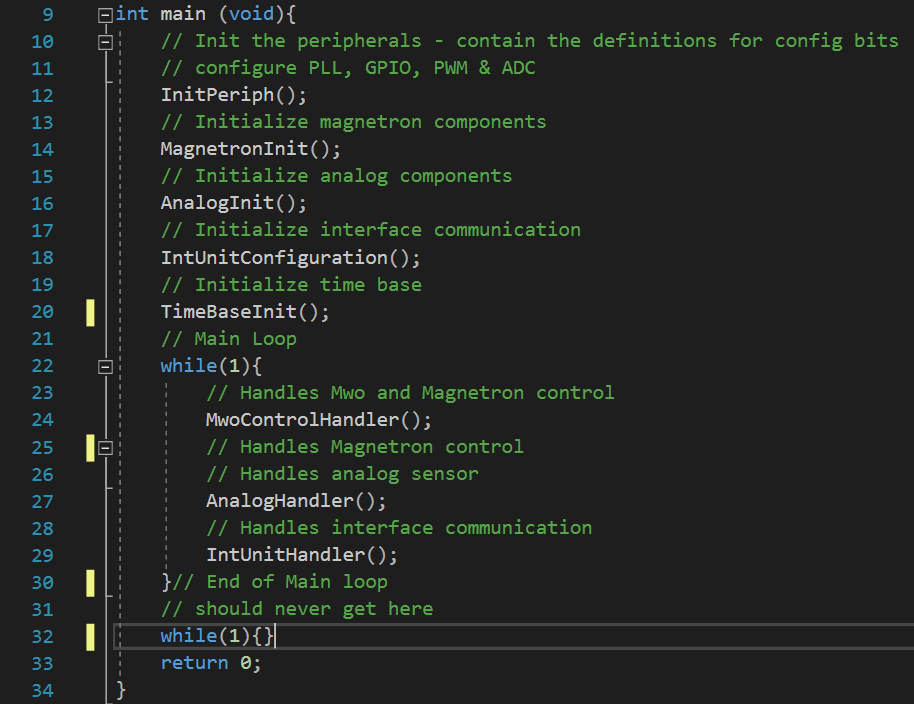
\includegraphics[width=1\textwidth]{./dados/figuras/func_main}
    \fonte{Autoria própria (2019)}
    \label{fig:figura-func-main}
\end{figure}

A função principal consiste apenas na inicialização dos periféricos do circuito e no laço de repetição que chama os manipuladores desenvolvidos.

No algoritmo, parâmetros de mínimos e máximos foram definidos de modo a possibilitar o controle do \textit{set-point} dentro de alguns limites de potência. Definiu-se que a frequência de chaveamento deve estar entre 20 kHz e 45 kHz, devido ao limite audível e a resposta em frequência dos componentes. Já quanto à potência, foi estipulado que deve estar entre 400 W e 1600 W, para possibilitar uma operação segura e contínua do magnetron.

\subsubsection{Controlador PI}
Para determinar o controlador do projeto, foram considerados controladores que pudessem responder de forma adequada à uma variável de processo que é regida por uma função de transferência que é muito difícil de se determinar. Assim, decidiu-se que, ao invés de calcular um controlador com função de transferência específica para a planta, iria utilizar-se um controlador mais flexível. Devido às altas frequências do circuito, e a natureza das grandezas que se deseja controlar, o controlador PI foi utilizado neste projeto. Este controlador permite um controle rápido, estável e apresenta menor \textit{overshoot} em relação à um controlador integral, além de possuir erro zero em estado estacionário, no caso de se desejar utilizar potência constante. O algoritmo do controlador PI faz, de forma digital, o controle do \textit{set point} através da soma acumulada dos valores anteriores multiplicados pelas constantes de proporção integral somados com a componente proporcional da fórmula. Para determinar os valores das constantes, foi utilizado um método que também é comum no controle de motores elétricos, descrito no manual disponibilizado pela fabricante do microcontrolador DSPIC33 em \citeonline{Microchip}. Este método consiste em zerar o ganho da constante integrativa ($K_i$) e de forma manual, através da variação da constante proporcional ($K_p$), alcançar uma resposta aceitável em questão de tempo e \textit{overshoot}. Determinando-se $K_p$, a constante $K_i$ é habilitada com valor aproximadamente 10 vezes menor que $K_p$. Em seguida, realiza-se ajustes finos manuais, de forma a se determinar $K_i$, de acordo com a ausência de \textit{overshoot} e um tempo de resposta de saída que é compatível com os requisitos do sistema. O algoritmo foi implementado na linguagem \textit{Assembly} para uma melhor performance, porém será exposto neste trabalho em C, da maneira em que foi idealizado:

\begin{figure}[H]
    \centering
    \caption{Algoritmo em C do controlador PI}
    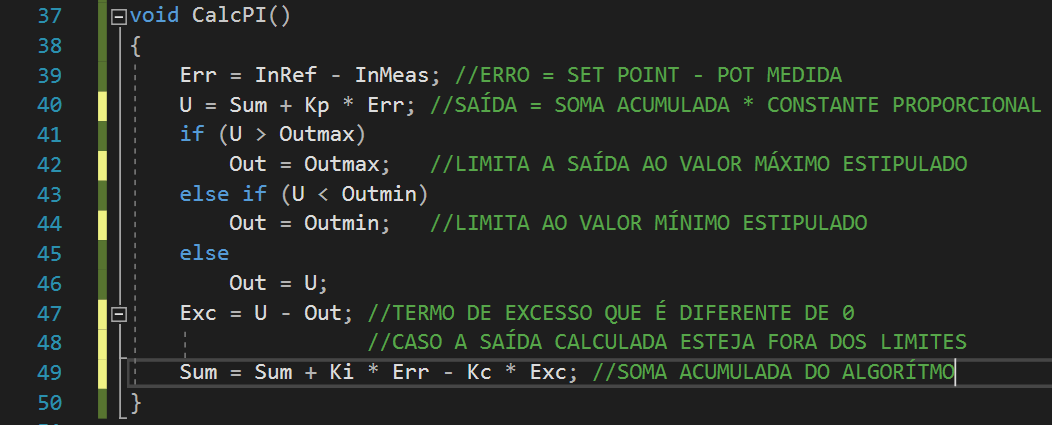
\includegraphics[width=1\textwidth]{./dados/figuras/func_pi}
    \fonte{Autoria própria (2019)}
    \label{fig:figura-func-pi}
\end{figure}

\subsubsection{Interrupções do Conversor AD}
Estas interrupções são disparadas a cada 30 $\mu$s, e os manipuladores desenvolvidos para esta interrupção lêem o nível do sinal analógico convertido e fazem o cálculo para o valor analógico equivalente, de acordo com os coeficientes de ajuste calculados. O valor calculado é atribuído à variáveis globais que são utilizadas nos demais algoritmos do sistema. A figura \ref{fig:figura-irq_ad} detalha os manipuladores:

\begin{figure}[H]
    \centering
    \caption{Manipulador desenvolvido}
    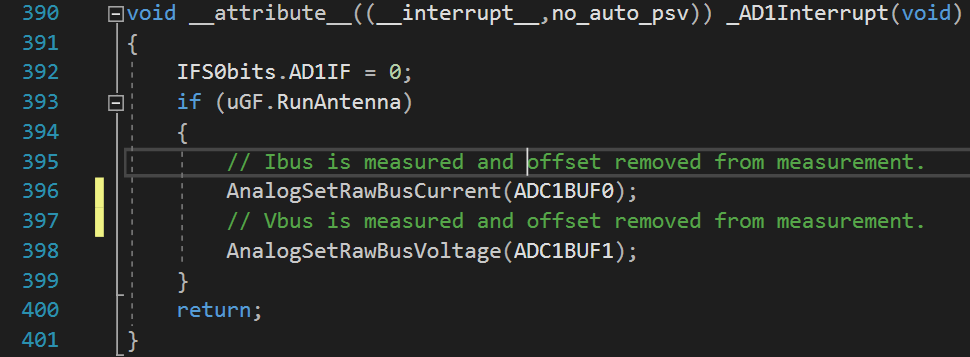
\includegraphics[width=1\textwidth]{./dados/figuras/irq_ad}
    \fonte{Autoria própria (2019)}
    \label{fig:figura-irq_ad}
\end{figure}


\subsubsection{Interrupção de \textit{input capture}}
Esta interrupção é acionada quando uma borda de subida ou descida é detectada pelo pino de entrada. O sinal de entrada deste pino é o sinal de controle que vem do circuito de comunicação. O manipulador desenvolvido para esta IRQ verifica se a borda detectada é de subida ou descida e conta o intervalo de tempo em que o sinal está alto e o intervalo de tempo em que o sinal está baixo. Os valores de sinal alto e baixo representam a potência solicitada pelo controlador para regular a potência de saída do magnetron. Esta interrupção também chama uma função que sinaliza que a realimentação está funcionando, a qual será detalhada na subseção da interface de comunicação. A figura \ref{fig:figura-irq_ic} contém o algoritmo desenvolvido para esta interrupção:

\begin{figure}[H]
    \centering
    \caption{Maniuplador desenvolvido}
    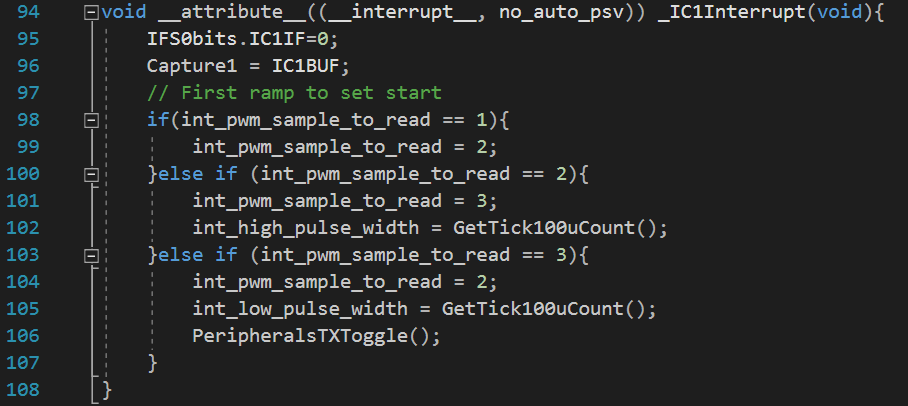
\includegraphics[width=1\textwidth]{./dados/figuras/irq_ic}
    \fonte{Autoria própria (2019)}
    \label{fig:figura-irq_ic}
\end{figure}


\subsubsection{Algoritmo de acionamento do Magnetron}
Por ser um componente de alta potência que pode causar danos ao circuito ou a terceiros caso operado incorretamente, o magnetron possui um algoritmo de acionamento próprio que, baseado nas variáveis de entrada medidas pelo microcontrolador e no estado do programa, pode desligar, ligar ou proteger o componente, colocando-o em modo \textit{stand-by}. Para tomar a decisão, o algoritmo leva em consideração a tensão medida pelo conversor AD e o ciclo de trabalho requisitado pelo controlador. Inicialmente, o magnetron começa em estado inicial, o qual somente inicializa variáveis do controlador. Feito isso, o sistema vai para o estado \textit{stand-by}, e aguarda o início do acionamento por parte da interface de usuário. Quando o acionamento é realizado, o algoritmo vai para o estado "rodando", o qual realiza o controle PI, faz verificações de segurança, mede os valores atuais de ciclo de trabalho e frequência e atribui novo ciclo de trabalho e frequência de acordo com o resultado obtido no algoritmo do controlador PI. A figura abaixo mostra o fluxograma do algoritmo desenvolvido:

\begin{figure}[H]
    \centering
    \caption{Algoritmo desenvolvido}
    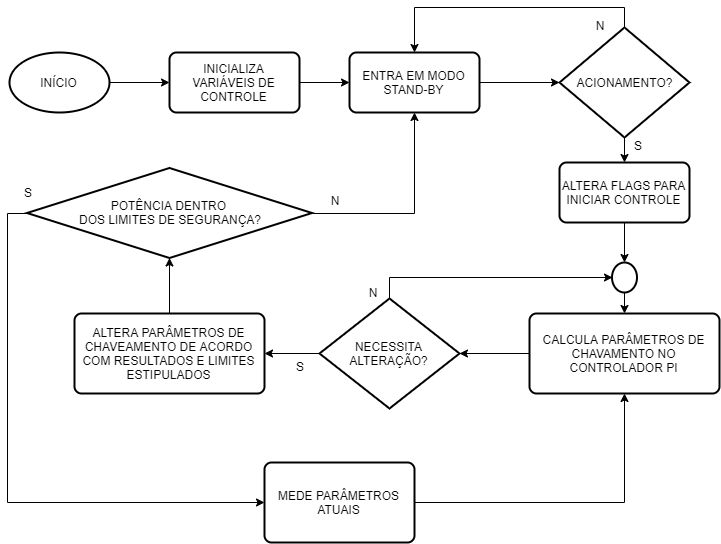
\includegraphics[width=1\textwidth]{./dados/figuras/mwo_flow}
    \fonte{Autoria própria (2019)}
    \label{fig:figura-mwo_flow}
\end{figure}

A figura a seguir detalha o código implementado:

\begin{figure}[H]
    \centering
    \caption{Impelementação do algoritmo de acionamento}
    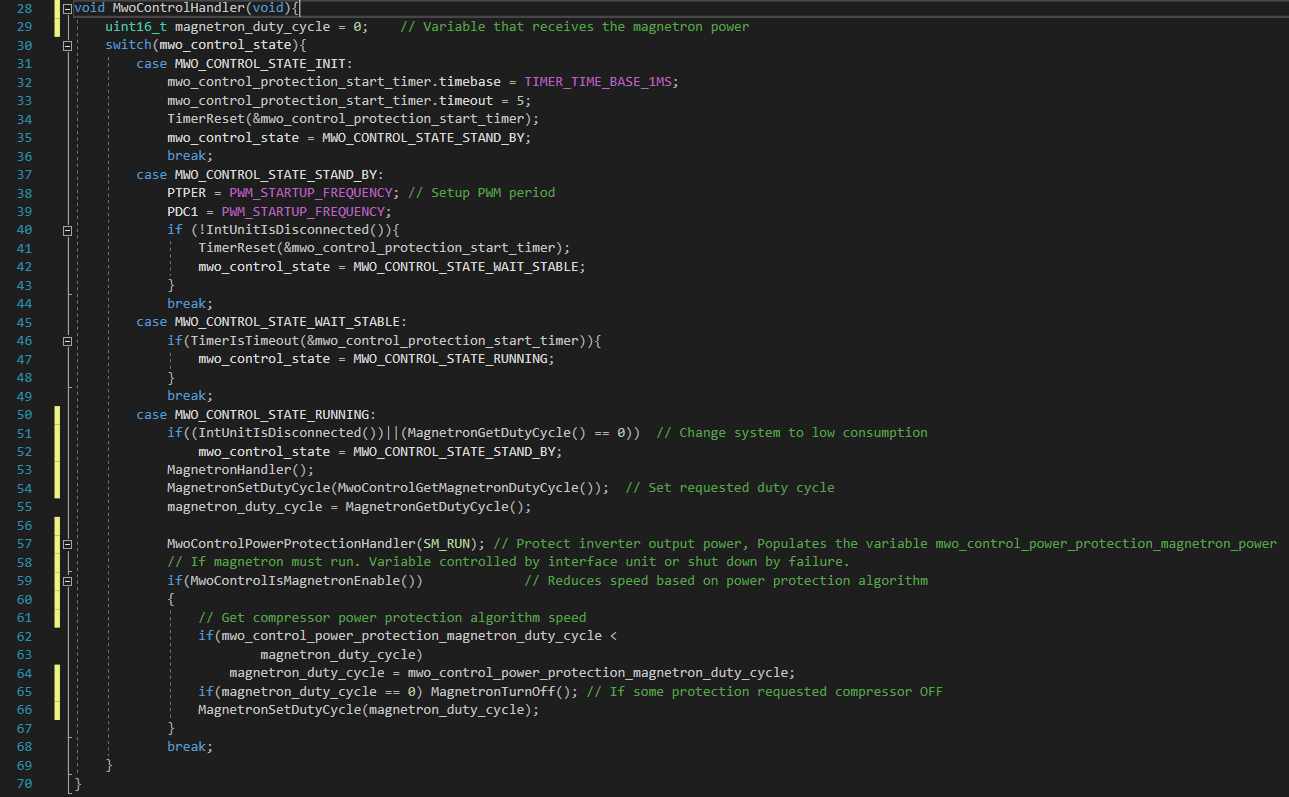
\includegraphics[width=1\textwidth]{./dados/figuras/func_mwo}
    \fonte{Autoria própria (2019)}
    \label{fig:figura-func_mwo}
\end{figure}

\subsubsection{Algoritmo de leitura do \textit{shunt} e da tensão de barramento}
Este algoritmo realiza as leituras dos valores medidos pelos conversores AD, e atribui os valores adquiridos à variáveis internas do sistema. Um temporizador é constantemente verificado para averiguar a necessidade de se tomar uma amostra. A frequência de amostragem foi definida em  5 kHz. Para adquirir os valores, o programa faz uma média móvel do valor medido e utiliza o resultado para determinar o valor da potência. Esta potência então é lida pelo controlador PI para fazer o controle da potência de saída do magnetron. Segue o algoritmo desenvolvido:

\begin{figure}[H]
    \centering
    \caption{Fluxograma do algoritmo}
    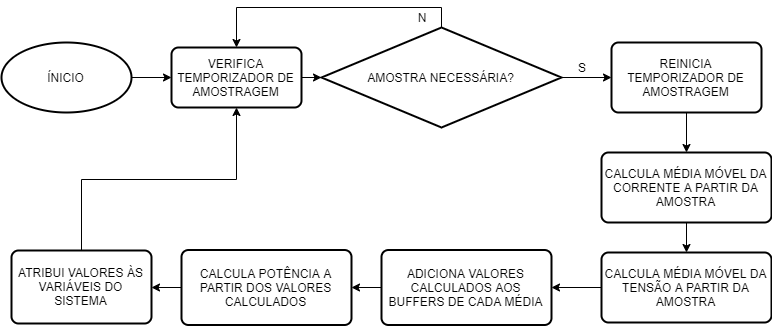
\includegraphics[width=1\textwidth]{./dados/figuras/flow_ad}
    \fonte{Autoria própria (2019)}
    \label{fig:figura-func_analog}
\end{figure}


\begin{figure}[H]
    \centering
    \caption{Implementação do algoritmo}
    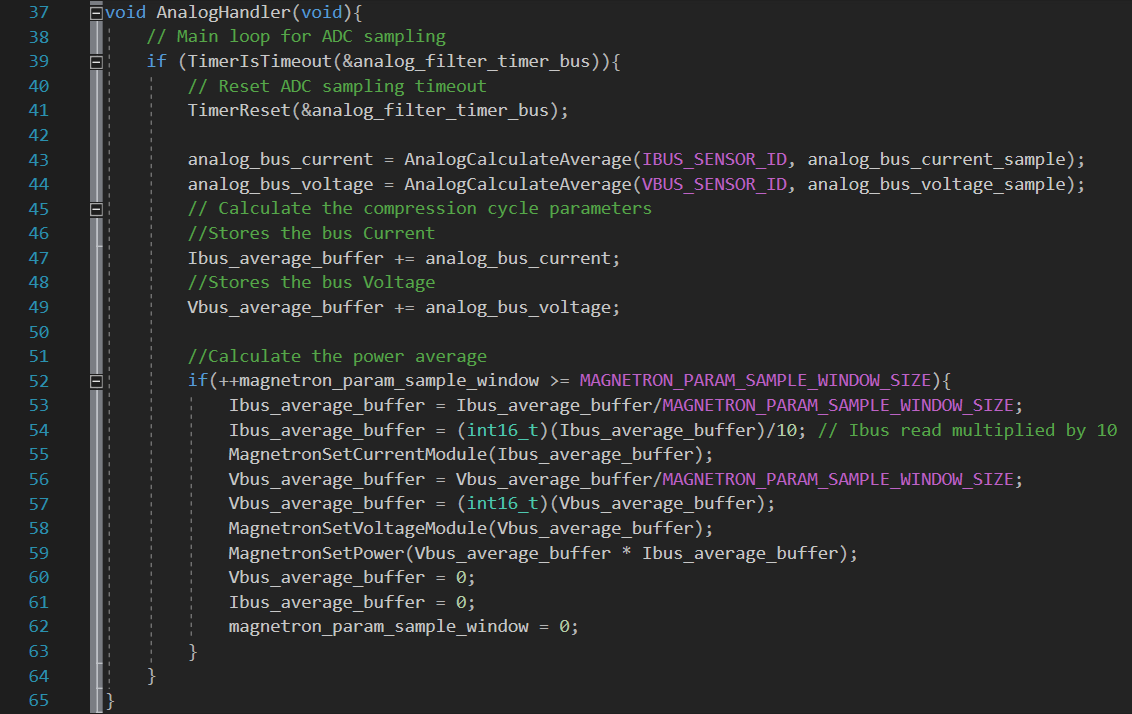
\includegraphics[width=1\textwidth]{./dados/figuras/func_analog}
    \fonte{Autoria própria (2019)}
    \label{fig:figura-func_analog}
\end{figure}



Para calcular a média móvel, foi desenvolvida uma função que calcula tanto para o sensor de corrente quanto para o sensor de tensão. Para diferenciar um do outro, apenas recebe um parâmetro com a identificação de qual que se quer fazer a média. A figura abaixo detalha a implementação em C da função desenvolvida:

\begin{figure}[H]
    \centering
    \caption{Função desenvolvida}
    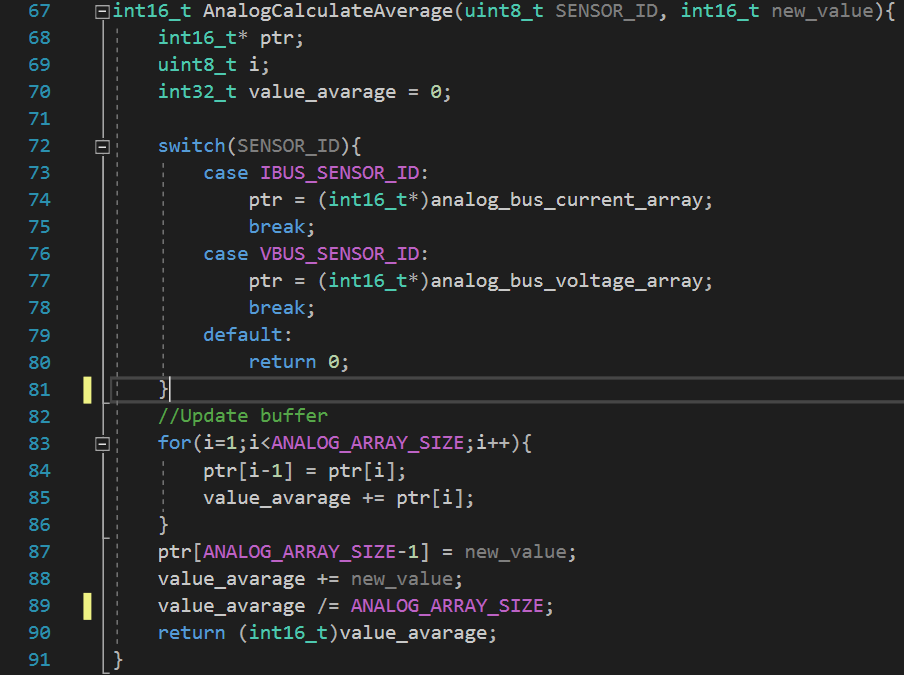
\includegraphics[width=1\textwidth]{./dados/figuras/func_average}
    \fonte{Autoria própria (2019)}
    \label{fig:figura-func_average}
\end{figure}


\subsubsection{Algoritmo da interface de comunicação}
O algoritmo desta função recebe como entrada  um sinal de frequência de 220 Hz, cujo ciclo de trabalho sinaliza o percentual de potência solicitada pelo magnetron e larguras de pulso são medidas pelo manipulador da interrupção de \textit{input capture}. Como saída, o algoritmo envia um sinal de status com metade da frequência do sinal de controle, e ciclo de trabalho fixado em 50\%, que é lido novamente no próprio microcontrolador. O sinal de status do sistema sinaliza se o magnetron está ligado e operante, com a realimentação de corrente funcionando. Este algoritmo contém dois estados de operação: Aguardando início e recebendo pacotes. No primeiro estado, a função verifica um temporizador que é reiniciado pelo sinal de controle. Quando o temporizador indica que há recebimento de sinal, o sistema é colocado no segundo estado. Neste estado, o algoritmo, através das larguras de pulso medidas pelo manipulador da interrupção, calcula o percentual de potência máxima solicitada pelo magnetron. Então, o programa atribui um novo ciclo de trabalho ao magnetron de acordo com o percentual calculado. Ou seja, esta função controla o \textit{set point} da planta. A figuras abaixo mostram o fluxograma e a respectiva implementação em C:
\begin{figure}[H]
    \centering
    \caption{Fluxograma desenvolvido}
    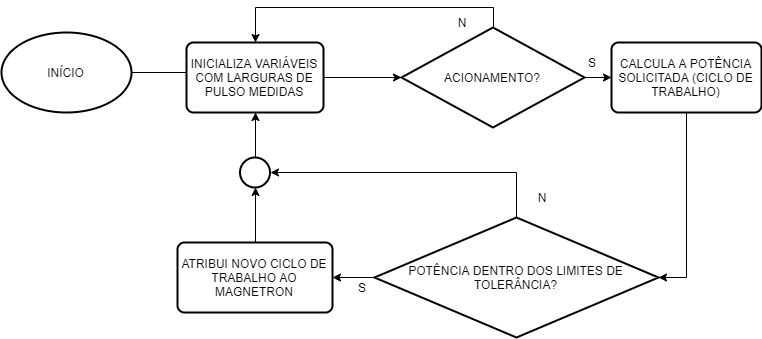
\includegraphics[width=1\textwidth]{./dados/figuras/flow_comm}
    \fonte{Autoria própria (2019)}
    \label{fig:figura-func_comm}
\end{figure}


\begin{figure}[H]
    \centering
    \caption{Função desenvolvida}
    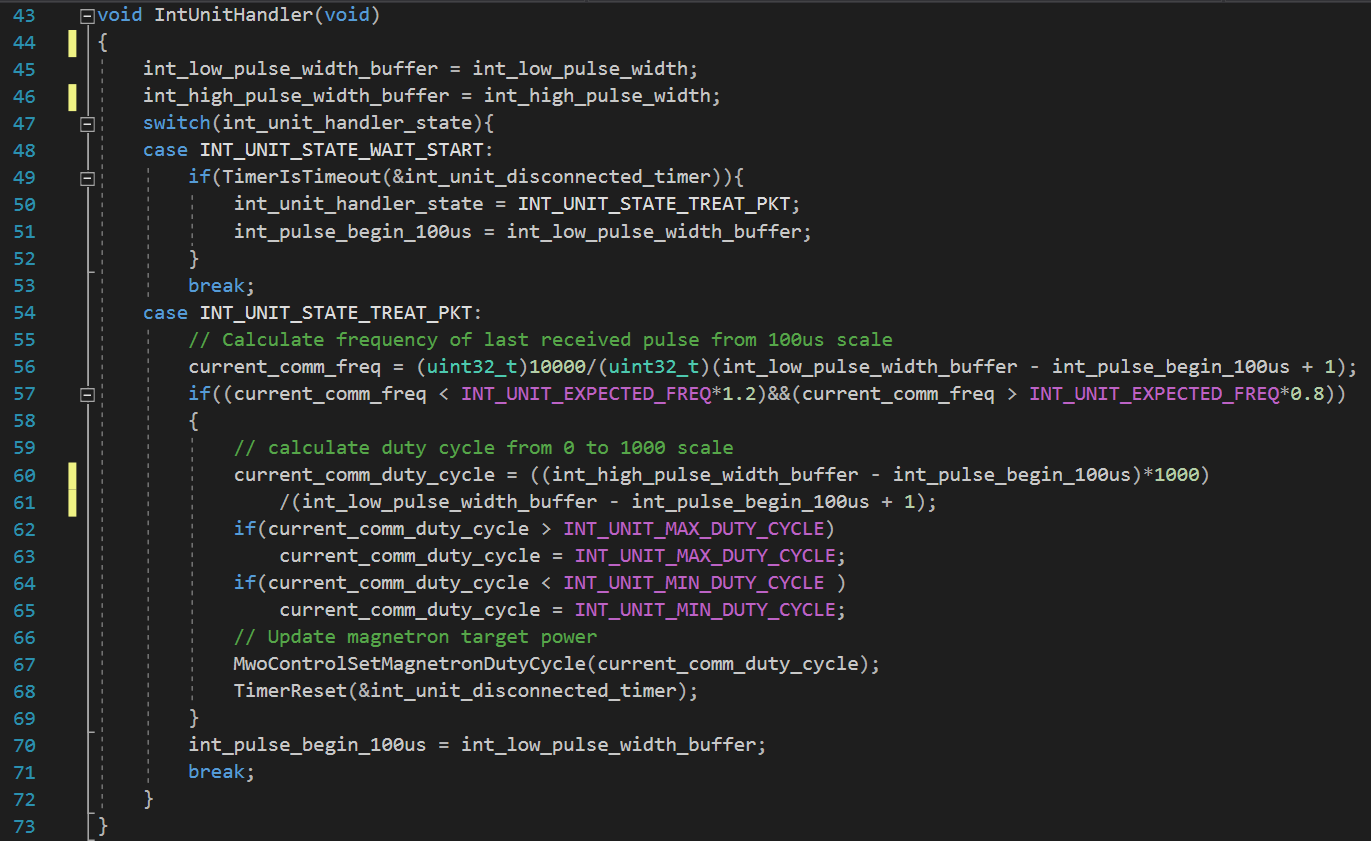
\includegraphics[width=1\textwidth]{./dados/figuras/func_comm}
    \fonte{Autoria própria (2019)}
    \label{fig:figura-func_comm}
\end{figure}